\section{\textit{CoppeliaSim}}
\label{sec:coppelia}

O \textit{CoppeliaSim} é um simulador de robôs que usa um mecanismo de cinemática para cálculos de cinemática direta e inversa e várias bibliotecas de simulação. Modelos e cenários são construídos pela montagem de vários objetos numa estrutura hierárquica.

Após ter sido feito o modelo \textit{CAD}, há duas etapas para a criação de um projeto em \textit{CoppeliaSim}: criar um modelo físico e adaptar os scripts \textit{Matlab} para controlo do robô. Posto isto, desenvolveu-se um modelo físico simples para testar a física do robô, como é possível observar na Figura \ref{fig:robo-fisico}.

Para o desenvolvimento deste modelo, é necessário criar uma forma primitiva. Neste caso foi utilizada a forma de cilindro para desenvolver o corpo do robô e as duas rodas. De seguida é necessário adicionar motores e sensores. Para a criação e ajuste da localização de cada peça foram utilizadas as ferramentas \textit{Object/item shift} e \textit{Scene Object Properties}. Sendo que se trata de um modelo físico, foi adicionada física, através da ferramenta \textit{Show dynamic properties dialog} em \textit{Scene Object Properties} às rodas do modelo, atribuídos valores aos motores e através da ferramenta \textit{Show volume parameters}, foram configurados todos os sensores. 
%
    \begin{figure}[!h] 
\centering
    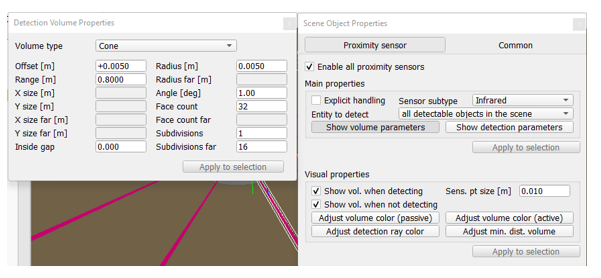
\includegraphics[width=0.8\textwidth]{./img/sens-prop}
  \caption{Propriedades dos sensores}% 
\label{fig:sensor-prop}
\end{figure}

        %
    \begin{figure}[!h] 
\centering
    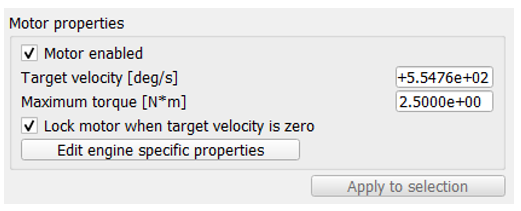
\includegraphics[width=0.6\textwidth]{./img/motor-prop}
  \caption{Propriedades dos motores}% 
\label{fig:motor-prop}
\end{figure}

        %
    \begin{figure}[!h] 
\centering
    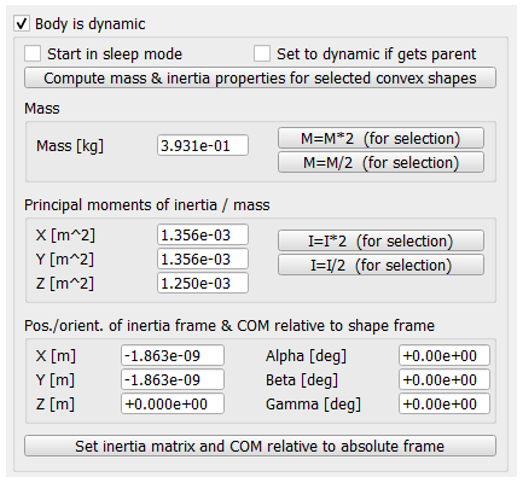
\includegraphics[width=0.6\textwidth]{./img/fisica-rodas}
  \caption{Física das Rodas}% 
\label{fig:rodas-fisica}
\end{figure}

Depois de testado o modelo físico, foi exportado o robô desenvolvido no \textit{Fusion} em formato \textit{.obj}, e inseriu-se este modelo no \textit{CoppeliaSim} sendo usado apenas como modelo gráfico, ou seja, serve apenas para visualizar. Isto pode ser feito através da ferramenta \textit{Common- Visibility} também em \textit{Scene Object Properties }. De seguida, ao robô obtido no \textit{CoppeliaSim}, adicionaram-se os sensores e foram colocados os elementos do robô de forma hierárquica para respeitar a física e comportar-se de acordo com o objetivo. Além disso foram utilizados cenários já desenvolvidos onde se colocou o robô e procederam-se testes para diversas situações. 
        %
    \begin{figure}[!h] 
\centering
    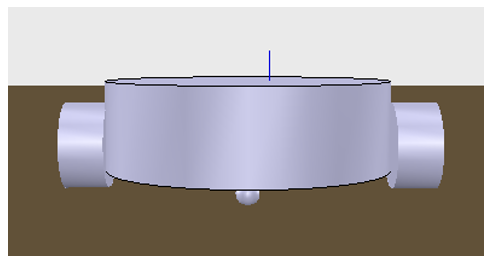
\includegraphics[width=0.7\textwidth]{./img/robo-copp}
  \caption{Modelo físico do robô}% 
\label{fig:robo-fisico}
\end{figure}

        %
    \begin{figure}[t] 
\centering
    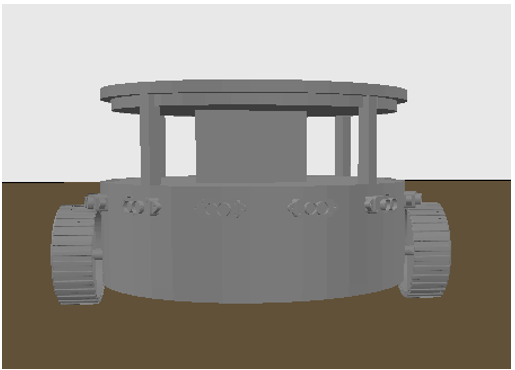
\includegraphics[width=0.7\textwidth]{./img/robo-copp-tot}
  \caption{Modelo total do robô}% 
\label{fig:robo-fisico-total}
\end{figure}